% LaTeX Template for a short article
% 
% To use:
%
% Copy into a new file, replace all
% [BRACKETED UPPER CASE TEXT]
% with your own, then run the latex command on it.
% Use dvips to print the .dvi output
\documentclass[DIV=10,BCOR=0cm]{scrartcl}
%\documentclass{article}
\usepackage{pslatex}
\usepackage{titling}
\usepackage[english,ngerman]{babel}
\usepackage[ansinew]{inputenc}
\usepackage{longtable}
\usepackage[colorlinks=false]{hyperref}
\usepackage{graphicx}


\author{Jan Petertonkoker
\texttt{janp@mail.upb.de}
}

\title{Thesen-Kritik-Replik-Verfahren - Datenstruktur}

\begin{document}

\setlength{\droptitle}{-80pt}
\maketitle

\pagestyle{plain}

\noindent
Dieses Dokument ist eine Beschreibung der Datenstrukturen, die der koaLA-/bidOWL-Extension zum Thesen-Kritik-Replik-Verfahren zugrunde liegen. In Abschnitt \ref{containerstruktur} wird zun�chst die Containerstruktur eines TKR-Objekts beschrieben. Danach folgt in Abschnitt \ref{attribute} eine Auflistung der verwendeten Attribute der verschiedenen Objekte.

\section{Containerstruktur}\label{containerstruktur}
Wenn eine neue Instanz des Thesen-Kritik-Replik-Verfahrens erstellt wird, wird ein Raumobjekt auf dem open-sTeam Server erstellt (typischerweise im Arbeitsraum einer Gruppe, in der das TKR-Verfahren durchgef�hrt werden soll). In diesem Raum werden weitere Container erstellt, um die Daten, die w�hrend der Durchf�hrung entstehen, strukturiert ablegen zu k�nnen. Abbildung \ref{container} zeigt diese Containerstruktur.

\begin{center} 
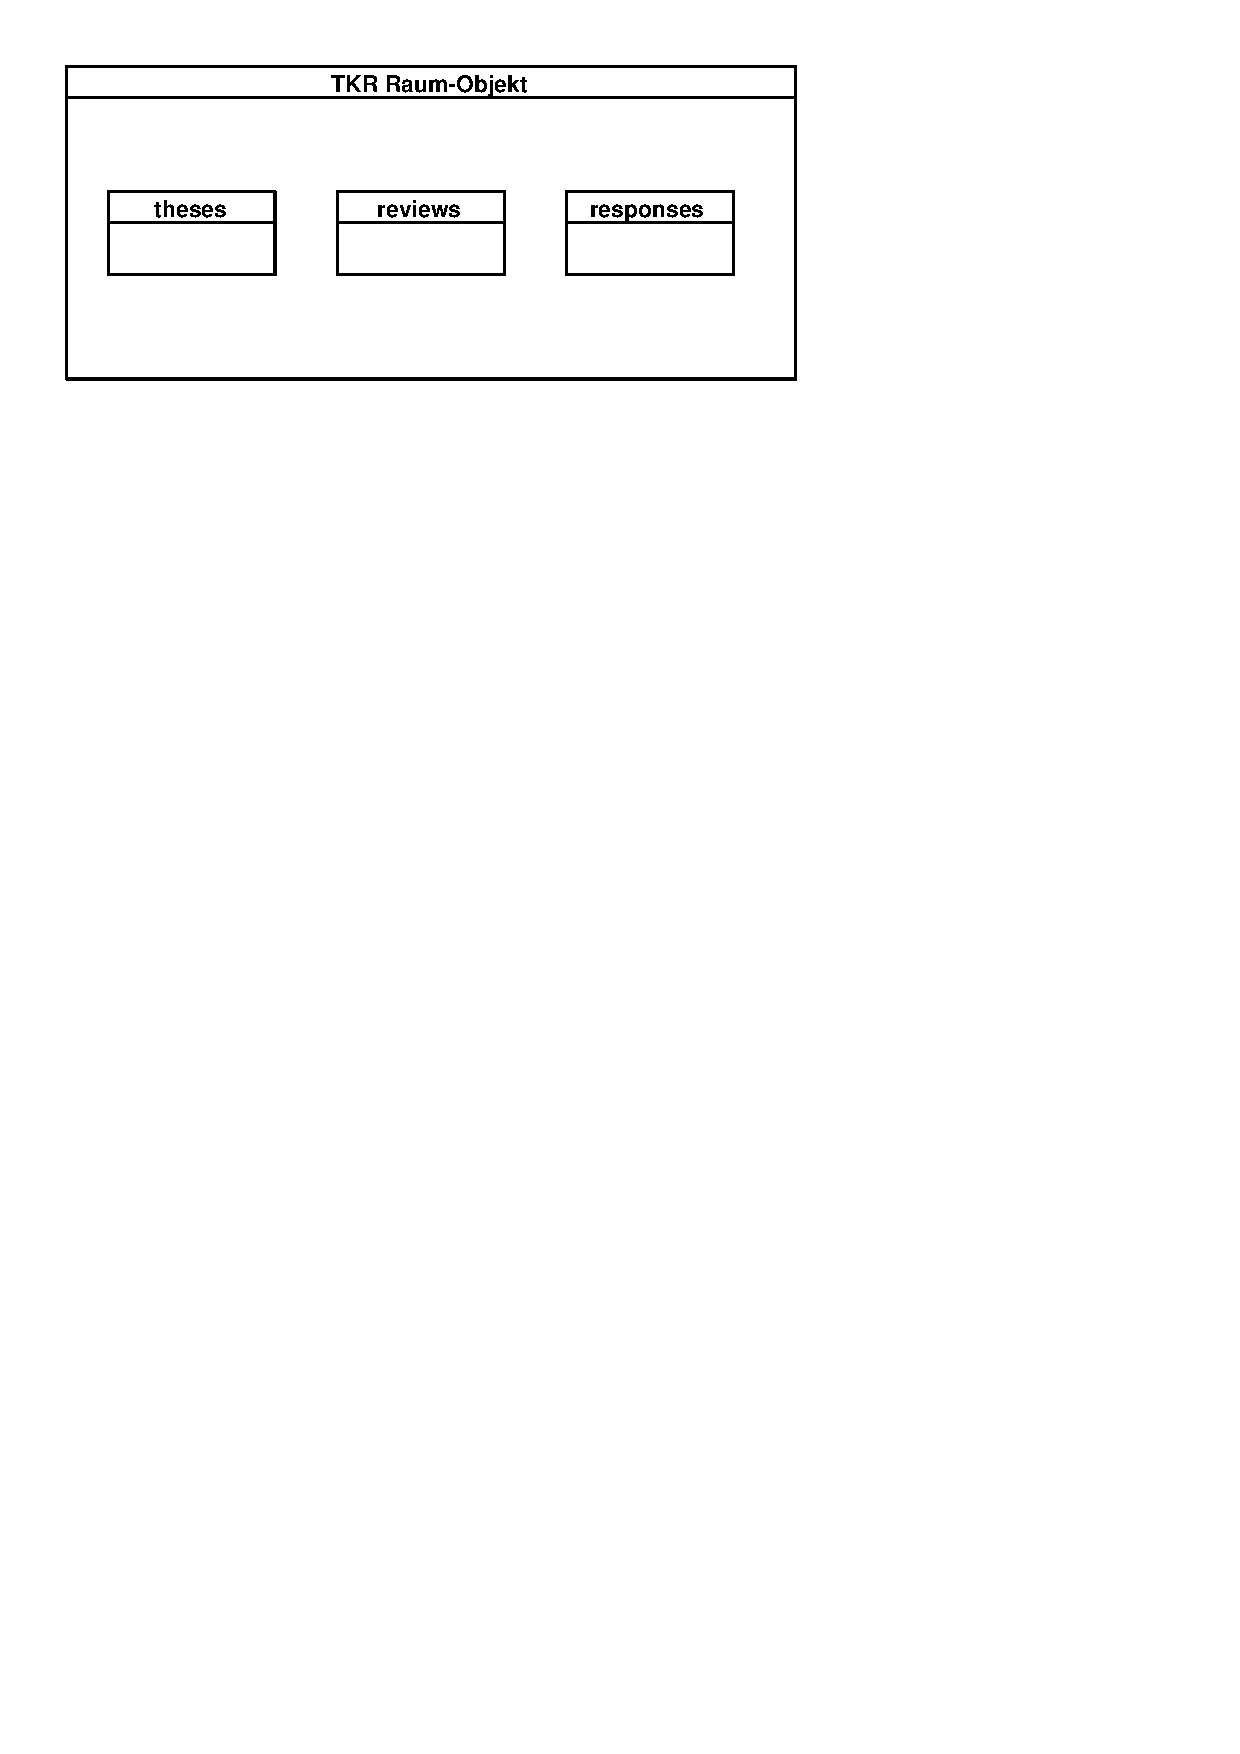
\includegraphics[scale=1]{images/container.pdf}
\captionof{figure}[Containerstruktur eines TKR-Raum-Objekts]{\label{container}Containerstruktur eines TKR-Raum-Objekts}
\end{center}

\noindent
Innerhalb des TKR-Raumobjekts werden also Container f�r die Thesen (Container "'theses"'), f�r die Kritiken (Container "'reviews"') und f�r die Repliken (Container "'responses"') erstellt. In diesen Containern werden w�hrend der Durchf�hrung die Thesen-, Kritik- und Replikobjekte abgelegt. Der Zusammenhang zwischen den verschiedenen Objekten wird in den jeweiligen Attributen gespeichert (siehe n�chster Abschnitt). Wenn zu einer These, Kritik oder Replik Dateien hochgeladen werden, wird ein neuer Container erstellt mit dem Namensschema "'ID\_files"' mit ID als Objekt-ID der These, Kritik oder Replik. Dort werden die hochgeladenen Dateien abgelegt. Dieser Container wird im zugeh�rigen Hauptcontainer ("'theses"', "'reviews"' oder "'responses"') angelegt.

\section{Attribute}\label{attribute}
Um das Thesen-Kritik-Replik-Verfahren durchf�hren zu k�nnen, m�ssen an den verschiedenen Objekten bestimmte Attribute gespeichert werden. Diese werden im Folgenden f�r die verschiedenen Objektarten dargestellt.

\noindent
\textbf{Attribute des Raumobjekts}

\begin{longtable}{|p{6.9cm}|p{7cm}|}
\hline
\textsc{Name} & \textsc{Beschreibung} \\ 
\hline
\hline
OBJ\_TYPE & TCR\_CONTAINER\\
\hline
TCR\_ROUNDS & Anzahl der Runden\\
\hline
TCR\_ADMINS & Array mit OIDs der Administratoren\\
\hline
TCR\_USERS & Array mit OIDs der Teilnehmer\\
\hline
TCR\_GROUP & Gruppenobjekt der Gruppe, die das TKR-Verfahren durchf�hrt\\
\hline
\end{longtable}

\noindent
In den Attributen des Raumobjekts werden die grundlegenden Einstellungen der TKR-Instanz gespeichert. Dabei werden die Anzahl der Runden, die Leiter/Administratoren und die Teilnehmer abgelegt. Au�erdem wird dem Attribut "'OBJ\_TYPE"' der Wert "'TCR\_CONTAINER"' zugeordnet, der es m�glich macht, sofort zu erkennen, dass dieser Raum eine TKR-Instanz darstellt.

\medskip
\noindent
\textbf{Attribute eines Thesenobjekts}

\begin{longtable}{|p{6.9cm}|p{7cm}|}
\hline
\textsc{Name} & \textsc{Beschreibung} \\ 
\hline
\hline
TCR\_ROUND & zugeh�rige Runde\\
\hline
TCR\_REVIEWS & Array mit OIDs der Kritiker (aktuell implimentiert: ein Kritiker pro These) und jeweils zugeordnet der OID des jeweiligen Kritikobjekts\\
\hline
TCR\_RELEASED & wenn ver�ffentlicht timestamp der Ver�ffentlichung; sonst 0\\
\hline
TCR\_FILES & ID des Containers in dem zugeh�rige Dateien abgelegt werden\\
\hline
\end{longtable}

\noindent

\medskip
\noindent
\textbf{Attribute eines Kritikobjekts}

\begin{longtable}{|p{6.9cm}|p{7cm}|}
\hline
\textsc{Name} & \textsc{Beschreibung} \\ 
\hline
\hline
TCR\_RESPONSE & OID des zugeh�rigen Replikobjekts\\
\hline
TCR\_RELEASED & wenn ver�ffentlicht timestamp der Ver�ffentlichung; sonst 0\\
\hline
TCR\_FILES & ID des Containers in dem zugeh�rige Dateien abgelegt werden\\
\hline
\end{longtable}

\medskip
\noindent
\textbf{Attribute eines Replikobjekts}

\begin{longtable}{|p{6.9cm}|p{7cm}|}
\hline
\textsc{Name} & \textsc{Beschreibung} \\ 
\hline
\hline
TCR\_RELEASED & wenn ver�ffentlicht timestamp der Ver�ffentlichung; sonst 0\\
\hline
TCR\_FILES & ID des Containers in dem zugeh�rige Dateien abgelegt werden\\
\hline
\end{longtable}

\end{document}

